\documentclass[conference]{IEEEtran}

\usepackage{amsmath}
\usepackage{url}
\usepackage{cite}
\usepackage{graphicx}


% correct bad hyphenation here
% \hyphenation{op-tical net-works semi-conduc-tor}


\begin{document}

\title{Generation T --- Pronounceable Password Generation Gamified\\
CPEN 442 Project Proposal}


% author names and affiliations
% use a multiple column layout for up to three different
% affiliations
% % % % CHANGE: Add your aliases here
% \author{\IEEEauthorblockN{blue, v6q8}
% \IEEEauthorblockA{Department of Computer Science\\
% University of British Columbia\\
% }
% \and
% \IEEEauthorblockN{Matt Labbe, hydro}
% \IEEEauthorblockA{Electrical and\\Computer Engineering\\
% University of British Columbia\\
% }
% }
\author{Group 16: Henry Li, Matthew Kuo, Kevin Lim, Anson Wong}


% make the title area
\maketitle

% As a general rule, do not put math, special symbols or citations
% in the abstract
\begin{abstract}
A study in gamified password generation is considered. The central idea is an extension on the memorability of pronounceable passwords. We use gamification as a means of introducing \emph{choice} and \emph{interaction} in near random generation of pronounceable passwords.
\end{abstract}

\section{Introduction}
% no \IEEEPARstart
Despite the plentiful amount of work on passwords done by the information security community, it remains an open issue. Secure and sufficiently unpredictable passwords are seemingly incompatible with their human counterparts, who will be the primary agents actively generating and using them. It is generally known that the more memorable the password, the more easily it will be compromised, since they rely on tricks such as passphrases and mnemonics, which allow them to be easily guessed using attacks such as a combinatorial attack. Further, it is ideal that users employ different passwords for each account they may use. Thus, we focus on the memorability of pronouncable passwords using a gamified generation approach. \emph{Gamification} is easily summarized as masking a primary, usually important or useful, but tedious or difficult, task while leveraging some specially designed leisurely or enjoyable task. Using this approach we want to investigate the role of interaction and choice on memorability in the hopes that longer, and thus more secure, passwords can be generated that remain useable. The system we designed will most likely be used to complement existing password aids such as password managers where, regardless of its ability to store and proffer passwords when needed, users must still memorize at least one password. The hope is that this particular password is memorable, as unpredictable as possible and stored locally on client hardware 
% or, for more savvy users, backed up safely for retreival
.

\section{Related Work}
What first inspired to use \emph{atomic} fragments of language called phonemes was work done by Lau et al. \cite{report:phonemes}. This resource also provided some phoneme sets such as the consonant sounds {\tt b, c, d, f, g, h, j, k, l, m, n, p, r, s, t, v, w, x, y, z, bl, br, dr, ch, cr, dr, fl, fr, gr, gl, pl, pr, qu, sh, sl, sp, st, sw, th, tr} concatenated with a vowel sound following. This lead quickly to the idea of actions deriving substrings as needed in a gamified task. 

Previous work in tools that buttress memorability of passwords such as mnemonic generation schemes Jeyaraman and Topkara \cite{report:mnemonic} is an example. However, in their opening discussion, White et al. \cite{report:prounounceability} underscore the importance of adversarial analysis in the design of password generation tools. White et al. present work by Kuo et al. \cite{report:mnemonicanalysis} which featured simulated dictionary attacks whose results suggested that dictionaries containing entries that are enumerated based on mimicing the mnemonic generation process could likely compromise the effectiveness of mnemonic schemes in terms of security. 

This emphasizes the parallel march of adversaries alongside the advancement in password generation schemes---as password generators become	more sophisticated, so too can adversaries use and emulate such generators' rules to construct dictionaries to attack the produced passwords. To increase the space and complexity of possible generated passwords, White et al. also develop methods to produce lexical neighbours of pronounceable strings. The basis of their work is a modified model by Bisani and Ney \cite{report:graph2phone} which converts graphemes to phonemes---the task of finding the pronounciation of a word (or string in the modified model) given its textual form. 

White et al. used the Carnegie Mellon University Pronouncing Dictionary \cite{report:CMUPD}, which is essentially a useful encoding of vocal speech in a textual form, as a dataset to train their model that rates a string's prounounceability using the path probability, a product of two conditional probabilities given string spelling and pronounciation.

We consider the objectives of Huh et al. \cite{report:surpass} in their quite recent work \emph{Surpass} to be distinctly comparable to ours. In their studies, they allow users to perform in-place replacement of characters in a randomly generated strings to be used as their passwords. In the user study, they employ the Atkinson-Shiffrin model of memory and thus the user study partitioned into initial generation and memory tests followed by a brief spell before reconvening to evaluate user recall of the password. Due to the similarities and the rigor of their user study, we feel that it's prudent to evaluate our method against a similar study outline. Though pragmatically, due to our heavy time constraints and in-person evaluations (rather than use of Mechanical Turk), we may make adjustments as necessary. 


% Next, we considered some heuristics to determine and measure prounounceability in White et al. \cite{report:prounounceability} which will be useful in scoring putative passwords and possibly influence the assignment of phonemes to blocks. Finally, we consider the alternative of mnemonic password derivation in \cite{report:mnemonic} as well as the evaluation design. 
\section{Methodology}
We attempt to modify the popular game \emph{Tetris} since we consider its mechanics are well known by users of computing devices and thus the procedure will be nearly self explanatory. The modifications reside in the encoding of phonemes which are randomly assigned to each block (refer to Figure \ref{tet}) of a tetromino. As lines are cleared, the phonemes associated to the blocks involved in the lines construct putative strings which will then be ranked and suggested to the user. We believe that this approximates a random process: the blocks are given random phonemes and the user, in playing the game offers another source of entropy. However, the principle interest lies in the latter---does the user's interaction with this system afford better memorability than a fully automated random process?
\subsection{Hyptheses}
Along those lines, the study is further driven by the following questions:
\begin{enumerate}
	\item Does user participation and interaction admit more memorability than a randomly generated password?
	\item Does user awareness of how their actions affect the produced password affect memorability in any meaningful way?
	% \item 
\end{enumerate}
\subsection{Polices}
Due to the short time and thus limited population in which we get to conduct our study, we have minimized it to feature two polices. 
% We have both groups memorize a random password and then
\begin{enumerate}
	\item {\bf\tt visible.} Our first policy allows the participant to see the phoneme representation of the tetromino blocks. 
	\item {\tt opaque.} Our second policy will mask the phoneme strings from the participant to test hypothesis 2.
	% \textbf{visible}
	% One group will have the phoneme representation of the blocks visible while generating the 
\end{enumerate}
Regardless of assigned policy, each participant will be subject to memorization of a password generated through pure random means.
\subsection{User Study Design}
We evaluate the policies with experiments involving friends and colleauges. The standard outcome of a trial game is that 5 passwords are produced, that is, each participant plays the game until they have cleared 5 lines. They may, however, continue to play until they are satisfied with a password selection. Following the footsteps of Huh et al. \cite{report:surpass}, the foundation of our experiment is the Atkinson-Shiffrin memory model. The first half of the experiment ensures that the passwords enter the short term memory of the participants and the latter half assesses the ``first-test memorability'' of passwords. The time separation between the first and second halves is two days. The rationale behind the separation duration is well expressed by Huh et al.: there are some enviroments in which users will be expected to perform password recall daily---though they may not have to during a weekend. Hence, the two day separation exhibits some realism.
% \subsubsection{Part 1}

\noindent{\bf Part 1: Tetris}
\begin{enumerate}
	\item \textbf{Password Setup:} Each participant was given a policy at random. Due to time constraints, however, we may have to later assign based on even representation. Each participant would play the game until at least 5 lines were cleared. 
	\item \textbf{Password Memorization:} Participants would then be asked to input the correct password 3 times to rehearse and aid in memorization. This rehearsal would conclude only when the participant entered the password correctly 3 times. 
	\item \textbf{Intermission:} For a bit of a palette cleanser, the participants will be asked to do a small word search. We use a generator provided by Discovery \cite{report:wordsearch}.
	\item \textbf{Password Entry (first trial):} Each participant is asked to enter the password they have chosen in step 1 and rehearsed in step 2. 
	% They will be given 3 chances.
\end{enumerate}

\noindent{\bf Part 2: Pure Random}
\begin{enumerate}
	\item \textbf{Password Setup:} Each participant is given a random password. We try to assign passwords of similar length and entropy as those produced using the gamified task for a useful comparison.
	\item \textbf{Password Memorization:} Similar to \emph{Part 1}, participants would be subject to a rehearsal which would conclude when the participant entered the password correctly 3 times. 
	\item \textbf{Intermission:} Similar to \emph{Part 1}, participants will be asked to do a small word search. 
	\item \textbf{Password Entry (first trial):} Each participant is asked to enter the password they have chosen in step 1 and rehearsed in step 2. 
	% They will be given 3 chances.
\end{enumerate}

\noindent{\bf Part 3: Password Recall}
\begin{enumerate}
	\item \textbf{Password Entry (after 2 days):} Each participant is asked to enter the password they have chosen in parts 1 and 2.
	\item \textbf{Survey} The participant is asked whether they have used external storage of the passwords.  
	% They will be given 3 chances.
\end{enumerate}
\subsection{Data Collected}
\begin{itemize}
	\item All 5 passwords (generated from 5 cleared lines in the game; with the chosen password emphasized) and the randomly generated password.
	\item Time taken to clear 5 lines in the game
	\item Number of attempts made in the rehearsal trials.
	\item Time taken to enter passwords.
	\item Memorability results: in the rehearsal we record whether a correct entry had occurred for each attempt
	\item Survey response
\end{itemize}
\subsection{Empirical Security Analyses}
With all of the passwords stored and hashed using some representative (something that is used frequently ``in the wild'' for online accounts) function, we make an attempt to crack the passwords using \emph{hashcat} \cite{report:hashcat} and measure the number of attempts required and time taken to crack them.
% It is convincing that ultimately passwords should be memorable if they are to be secure, since if long passwords remain memorable, we can in principle construct arbitrarily long passwords that retain usability.
\begin{figure}[t]
	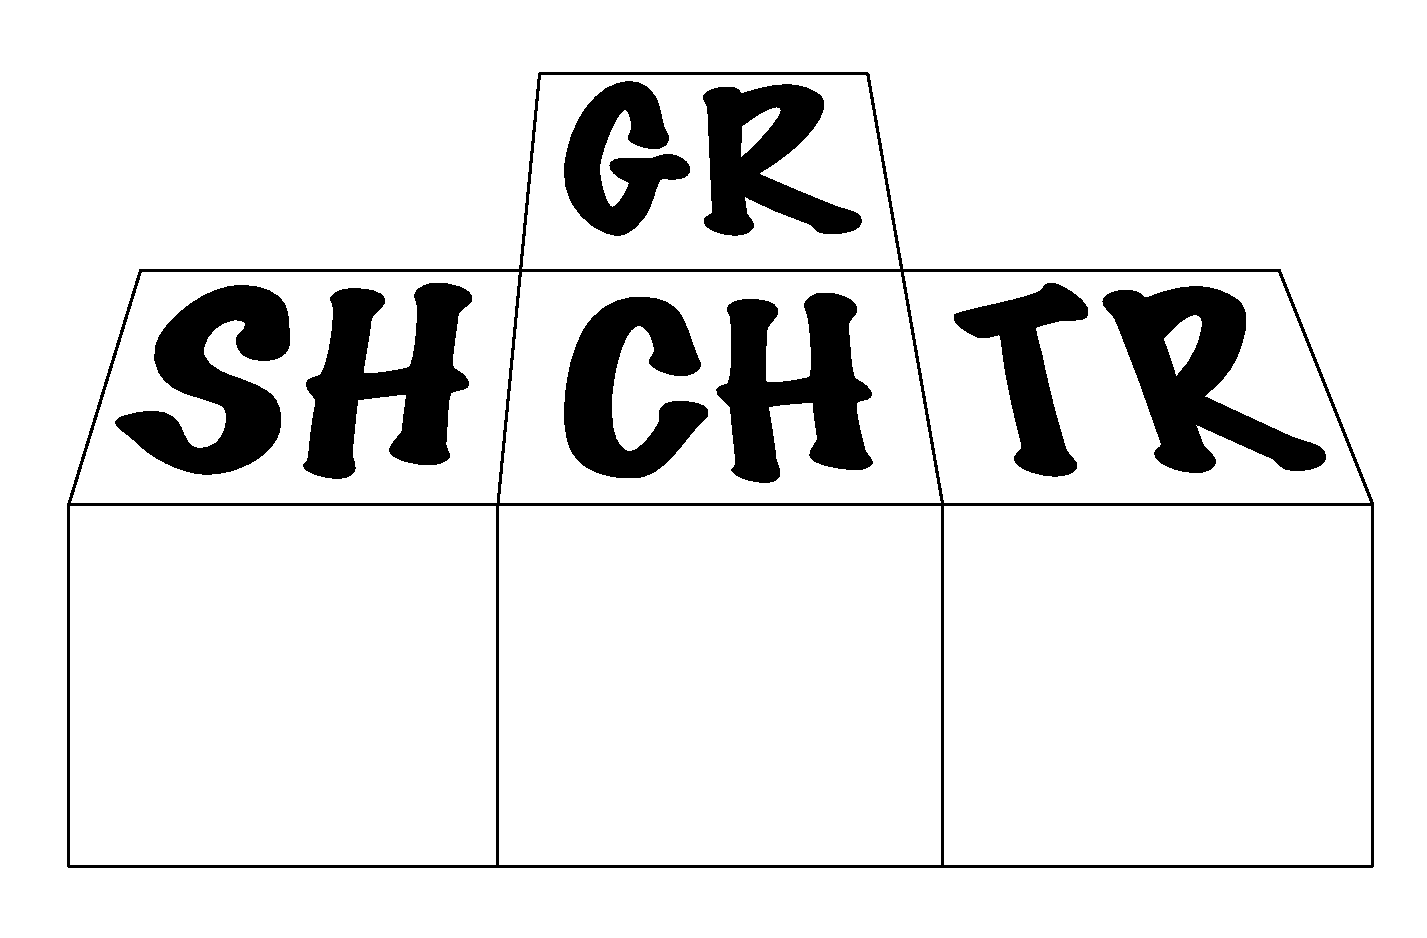
\includegraphics[width=.5\textwidth]{tetrophon.pdf}
	\caption{An example \emph{tetromino} whose phoneme representation is transparent.}
	\label{tet}
\end{figure}



% \section{Evaluation of Our Method}
% To investigate the effect of interaction in the password generation process, we will isolate two populations of subjects: one group will be aware of the phonemes while playing the game while the other will not have the random phonemes be transparent as an element of the game. After playing, the groups will be asked to memorize a chosen generated password. Both parties will also participate in a memory exercise in attempt to memorize a automatically generated random pronounceable password. We also time the entry of the passwords to effectively study the usability of the passwords generated with the various methods. Participants of this study will be asked to return for follow-up evaluation of password recall. We do not ask the users to produce their own passwords since we feel this would intorduce a hazard in that they may simply prefix or append suffixes to existing live passwords that they may be using actively to achieve better memorability. (??) Lastly, an empirical study on the strength of the passwords will be performed using GPU hashing. We choose a hash function representative of contemporary password storage methods. Strength will be based on how many attempts and how arduous it is to crack the collected passwords.

% \section{Timeline}
% We expect that a functional prototype should be built by the middle of November at the latest and we attempt to complete this phase as soon as possible to allow as much time as available to perform the studies and consequent analysis. We plan to allot approximately 2 weeks to perform the studies, perhaps completing some analysis concurrently wherever possible (some data may need the full sample size in order to be meaningful). We may feature a mock-interview session (done by members of our team) in a film to showcase the process in an enticing manner. Final report as well as poster and slides will hopefully be done by early December. 

\section{Future Work}
% We have limited time to commit to the studies but we hope our modest incursion into this genre of password generation will spark intrigue and propel further study.
Given more time, we would undoubtedly like to commit to doing studies with more participants. There is room to streamline the prototype for more automation in data recording and administering of the evaluation. To that regard, it would be sensible to construct the game from scratch. We had settled on using a Python implementation \cite{report:pytetris} since its data layout was more amenable to our modification goals than the comparable Javascript implmentations we found. However, we feel a handmade Javascript implmentation, with its ease in deployment, would be more amenable to larger scale studies that are warranted to evaluate our hyptheses fully.

Further, we would like to examine the effects on the difficulty of the game---and conversely, the effects of player skill in the generation process. Can more proficient players, whose more commanding control over the task, produce more memorable passwords? Do the memorability results, assuming they are positive, due to skill manifest simply due to less cognitive load in completing the task or game allowing their minds some latent ability to focus on the implicit memory task? Or do the interactions--the mapping between action and output--simply become more salient when one gains prowess over a task?

We feel there is more room to investigate the linguistic concerns raised by White et al. \cite{report:prounounceability} in their study of pronouncability. This interdisciplinary approach affects both the generation and analysis of password generation. We would firstly like to see if there is any advantage in training and implementing a model for scoring the putative passwords based on pronounceability rather than the quadgram log-likelihood score we currently use. Due to time, we were unable to commit to training the model described by White et al. but we see it beneficial in the interests of adversarial analysis. Using a confluence of work done by Huh et al. \cite{report:surpass} and White et al., one can easily imagine that phonetic replacements could come into play, increasing the entropy of the resultant password further, while perhaps affording better memorability to the user.

\section{Acknowledgements}
We are grateful for the guidance of Konstantin Beznosov in early iterations of concepts presented in this report. His insights have provided us confidence and curiosity in approaching this problem. 
\bibliographystyle{IEEEtran}
\bibliography{IEEEabrv,writeup.bib}
% \begin{thebibliography}{1}
% 	\bibitem{}
% \end{thebibliography}

% that's all folks
\end{document}


